% Digital Logic Report Template
% Created: 2020-01-10, John Miller

%==========================================================
%=========== Document Setup  ==============================

% Formatting defined by class file
\documentclass[11pt]{article}

% ---- Document formatting ----
\usepackage[margin=1in]{geometry}	% Narrower margins
\usepackage{booktabs}				% Nice formatting of tables
\usepackage{graphicx}				% Ability to include graphics

%\setlength\parindent{0pt}	% Do not indent first line of paragraphs 
\usepackage[parfill]{parskip}		% Line space b/w paragraphs
%	parfill option prevents last line of pgrph from being fully justified

% Parskip package adds too much space around titles, fix with this
\RequirePackage{titlesec}
\titlespacing\section{0pt}{8pt plus 4pt minus 2pt}{3pt plus 2pt minus 2pt}
\titlespacing\subsection{0pt}{4pt plus 4pt minus 2pt}{-2pt plus 2pt minus 2pt}
\titlespacing\subsubsection{0pt}{2pt plus 4pt minus 2pt}{-6pt plus 2pt minus 2pt}

% ---- Hyperlinks ----
\usepackage[colorlinks=true,urlcolor=blue]{hyperref}	% For URL's. Automatically links internal references.

% ---- Code listings ----
\usepackage{listings} 					% Nice code layout and inclusion
\usepackage[usenames,dvipsnames]{xcolor}	% Colors (needs to be defined before using colors)

% Define custom colors for listings
\definecolor{listinggray}{gray}{0.98}		% Listings background color
\definecolor{rulegray}{gray}{0.7}			% Listings rule/frame color

% Style for Verilog
\lstdefinestyle{Verilog}{
	language=Verilog,					% Verilog
	backgroundcolor=\color{listinggray},	% light gray background
	rulecolor=\color{blue}, 			% blue frame lines
	frame=tb,							% lines above & below
	linewidth=\columnwidth, 			% set line width
	basicstyle=\small\ttfamily,	% basic font style that is used for the code	
	breaklines=true, 					% allow breaking across columns/pages
	tabsize=3,							% set tab size
	commentstyle=\color{gray},	% comments in italic 
	stringstyle=\upshape,				% strings are printed in normal font
	showspaces=false,					% don't underscore spaces
}

% How to use: \Verilog[listing_options]{file}
\newcommand{\Verilog}[2][]{%
	\lstinputlisting[style=Verilog,#1]{#2}
}




%======================================================
%=========== Body  ====================================
\begin{document}

\title{ELC 2137 Lab 07: Binary Coded Decimal}
\author{Yiting Wang}

\maketitle


\section*{Summary}

In the last lab, we implemented a 7-segment display. We input numbers in binary, and it outputs in hex. When you get used to it, hex is fine to read, but it’s not as easy as decimal,  particularly for multi-digit numbers. In this lab, you will make a cheat button that will turn the display to decimal and then back to hex.  \\



\section*{Q\&A}

There is no question in lab7.\\



\section*{Results}

	Firgure 1 is the simulation waveform and ERT of the Add3.\\
	\begin{figure}[ht]\centering
		\begin{tabular}{l|rrrr|rrrr|rrrr|rrrr|r}
			Time (ns): & 0 & 10 & 20 & 30 & 40 & 50 & 60 & 70 & 80 & 90 & 100 & 110 & 120 & 130 & 140 & 150 \\
			\midrule
			num & 0000 & 0001 & 0010 & 0011 & 0100 & 0101 & 0110 & 0111 & 1000 & 1001 & 1010 & 1011 & 1100 & 1101 & 1110 & 1111 \\
			\midrule
			out & 0000 & 0001 & 0010 & 0011 & 0100 & 1000 & 1001 & 1010 & 1011 & 1100 & 1101 & 1110 & 1111 & 0000 & 0001 & 0010 \\
			\bottomrule
		\end{tabular}\medskip
		
		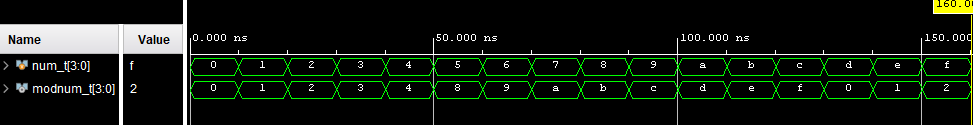
\includegraphics[width=1\textwidth]{add3_simulate}
		\caption{the simulation waveform and ERT of the 4-bit Multiplexer}
		\label{fig:add3_simulate}
	\end{figure}


Firgure 2 is the simulation waveform and ERT of the 6-bit BCD.
\begin{figure}[ht]\centering
	\begin{tabular}{l|rrr|rrr}
		Time (ns): & 0 & 10 & 20 & 30 & 120 & 130 & 140 & 150 \\
		\midrule
		num & 0000 & 0001 & 0010 & 1101 & 1110 & 1111 \\
		\midrule
		out & 0000 & 0001 & 0010 & 1111 & 0000 & 0001 & 0010 \\
		\bottomrule
	\end{tabular}\medskip
	
	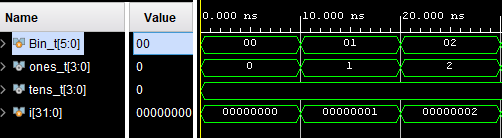
\includegraphics[width=1\textwidth]{bcd6_simulate_beginning}
	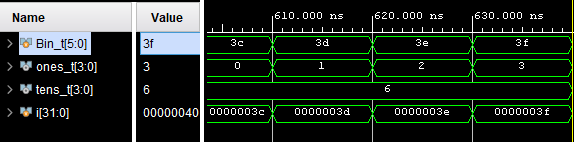
\includegraphics[width=1\textwidth]{bcd6_simulate_end}
	\caption{the simulation waveform and ERT of the 4-bit Multiplexer}
	\label{fig:add3_simulate}
\end{figure}


Firgure 1 is the simulation waveform and ERT of the Add3.
\begin{figure}[ht]\centering
	\begin{tabular}{l|rrrr|rrrr|rrrr|rrrr|r}
		Time (ns): & 0 & 10 & 20 & 30 & 40 & 50 & 60 & 70 & 80 & 90 & 100 & 110 & 120 & 130 & 140 & 150 \\
		\midrule
		num & 0000 & 0001 & 0010 & 0011 & 0100 & 0101 & 0110 & 0111 & 1000 & 1001 & 1010 & 1011 & 1100 & 1101 & 1110 & 1111 \\
		\midrule
		out & 0000 & 0001 & 0010 & 0011 & 0100 & 1000 & 1001 & 1010 & 1011 & 1100 & 1101 & 1110 & 1111 & 0000 & 0001 & 0010 \\
		\bottomrule
	\end{tabular}\medskip
	
	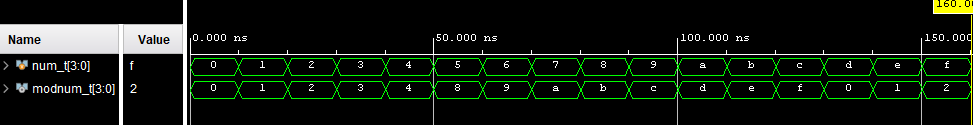
\includegraphics[width=1\textwidth]{add3_simulate}
	\caption{the simulation waveform and ERT of the 4-bit Multiplexer}
	\label{fig:add3_simulate}
\end{figure}


\section*{Code}

\subsection*{File Inclusion}
\Verilog[caption=Add3 Verilog code,label=code:file_ex]{add3.sv}

\subsection*{File Inclusion}
\Verilog[caption=Add3 Multiplexer Test Benches Verilog code,label=code:file_ex]{add3_test.sv}


\end{document}
